%%%
%% Design :: Database Design
%%%
\section{Database Design}
\label{sec:database_design}

As part of the testing strategy a list of clues and their solutions are required
to be stored. In order to accurately store a large amount of training data, a 
database will be used.

The database design is of a minimalistic approach as it is not intended to hold
a large amount of data, nor will it be used within a production environment. 
Figure \ref{fig:database_erd} shows the proposed database design.

Each record will contain a clue, a solution, and the solutions length. The
solutions length has been assigned a VARCHAR data type, because solutions can
span across more than one word. For example 3,4 would relate to two words, of
three and four characters respectfully. Each of these attributes are required 
--- i.e. not null.

The orientation attribute is an ENUM that contains either `down' or `up', 
indicating the direction that the solution is arranged. The orientation may be 
useful for certain clue types, such as reversal, where by the clue references 
the direction --- e.g. north-to-south, or east-to-west.

The clue number attribute stores the number of clue, as some clues use the clue 
number in obtaining the solution answer. Although this is uncommon, it will be 
taken into consideration.

The clue type attribute is an ENUM that holds the various types of clues, 
such as `purely cryptic' or `anagram'. It is intended that these values will be 
`mapped' to the system code, so that clues can be used automatically when 
training.

\begin{figure}[H]
  \centering
  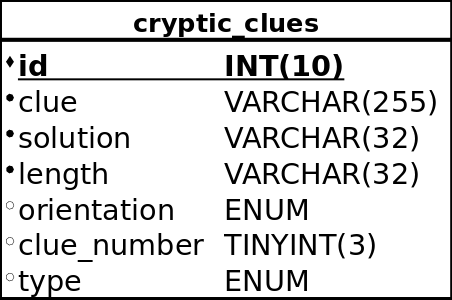
\includegraphics[scale=0.5]{database/database.png}
  \caption{Testing database entity-relationship diagram}
  \label{fig:database_erd}
\end{figure}
